\documentclass[letterpaper,12pt]{scrartcl}
\usepackage{epsfig,latexsym,amsmath,amssymb,epic,eepic,psfrag,subfigure,float,euscript,array}
\usepackage[latin1]{inputenc}
\usepackage[margin=24mm]{geometry}
\usepackage{enumitem}
\usepackage{tikz,pgf,pgfplots}
\usepgfplotslibrary{fillbetween}
\usepgfplotslibrary{groupplots}
\usetikzlibrary{decorations, arrows}

\usepackage[amssymb]{SIunits}

\newenvironment{exercise}[1][Problem]{\begin{trivlist} \item[\hskip
    \labelsep {\stepcounter{exerctr}\bfseries #1
      \arabic{exerctr}}]}{\end{trivlist}\vspace{10mm}}

\newcounter{exerctr}
\newcounter{abcctr}[exerctr]

\newcommand{\abc}{\noindent\vspace{1mm}\\ {\bf
    \stepcounter{abcctr}(\alph{abcctr})\ }}
\newcommand{\bbm}{\begin{bmatrix}}
\newcommand{\ebm}{\end{bmatrix}}
\newcommand{\point}[1]{\hfill {\bf (#1p)}\\ \vspace{-5mm}}
\newcommand{\ctrb}{\EuScript{S}}
\newcommand{\Lap}{\mathcal{L}}
\newcommand{\obsv}{\EuScript{O}}
\newcommand{\realdel}{\text{Re}}
\newcommand{\imagdel}{\text{Im}}
\newcommand{\bC}{\mathbb{C}}
\newcommand{\bR}{\mathbb{R}}
\newcommand{\bmpv}{\begin{minipage}[t]}
\newcommand{\bmps}{\begin{minipage}[t]{45mm}}
\newcommand{\bmpm}{\begin{minipage}[t]{90mm}}
\newcommand{\bmpl}{\begin{minipage}[t]{\textwidth}}
\newcommand{\emp}{\end{minipage}}
\newcommand{\mexp}[1]{\ensuremath{\mathrm{e}^{#1}}}
\newcommand*{\laplaceinv}[1]{\ensuremath{\mathcal{L}^{-1} \left\{#1\right\}}}
\newcommand*{\ztrf}[1]{\ensuremath{\mathcal{Z} \left\{#1\right\}}}

\newcommand{\AxisRotator}[1][rotate=0]{%
    \tikz [x=0.2cm,y=0.60cm,line width=.1ex,-stealth,#1] \draw (0,0) arc (-150:150:1 and 1);%
}

\newcommand{\shift}{\ensuremath{\operatorname{q}}}
%\addtolength{\topmargin}{-1cm}
%\textheight 22.5cm
%\oddsidemargin 1.3cm
%\evensidemargin 1.3cm

\makeatletter
\newcommand*{\rom}[1]{\expandafter\@slowromancap\romannumeral #1@}
\makeatother

\newcommand*\circled[1]{\tikz[baseline=(char.base)]{
            \node[shape=circle,draw,inner sep=2pt] (char) {#1};}}


\pgfplotstableread[col sep=comma]{inputs.dat}\inputtable
\pgfplotstableread[col sep=comma]{responses.dat}\outputtable

\title{Computerized Control partial exam 1 (18\%)}
\author{Kjartan Halvorsen}
\date{}

\begin{document}

\maketitle


\begin{description}
\item[Time] September 12 19:05-20.35
\item[Place] 4203
\item[Permitted aids] The single colored page with your own notes, table of Laplace transforms, calculator
\end{description}

All answers should be readable and well motivated (if nothing else is written). Solutions/motivations should be written on the provided spaces in this exam. Use the last page if more space is needed.

\begin{center}
{\Large Good luck!} \\
\end{center}

\noindent
\fbox{
\bmpl
{\bf Matricula and name:}\\
\vspace*{14mm}
\emp}


%\clearpage

%-----------------------------------------------------------------

\subsection*{Control of a frictionless mechanical system}
Friction is ubiquous in mechanical systems, but can sometimes be neglected in a model. The textbook gives one such example: Control of the position of the arm of a hard disk drive. With the input signal $u(t)$ being the torque applied to the arm, $y(t)$ the angular position of the arm and $J$ its moment of inertia, the system is described by the differential equation
\begin{equation}
 J\ddot{y}(t) = u(t).
\label{eq:ode}
\end{equation}

\begin{center}
  \begin{tikzpicture}[node distance = 2cm]
    \node (image) {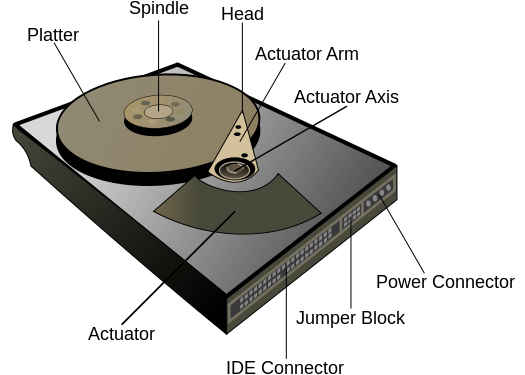
\includegraphics[width=0.36\textwidth]{../../figures/hard-drive.png}};

    \node[coordinate, right of=image, node distance=5cm] (input) {};
    \node[draw, right of=input] (block) {$G(s) = \frac{1}{Js^2}$};
    \node[coordinate, right of=block] (output) {};
    
    \draw[->] (input) -- node[above] {$u(t)$} (block);
    \draw[->] (block) -- node[above] {$y(t)$} (output);
  \end{tikzpicture}
\end{center}


\begin{exercise}

\abc
Show that zero-order-hold sampling of the model \eqref{eq:ode} gives the pulse-transfer function
\[ H(z) = \frac{\frac{h^2}{2J}(z+1)}{(z-1)^2}. \] 

\noindent
\fbox{
\bmpl
{\bf Calculations:}\\
\vspace*{135mm}
\emp}

\abc State as a mathematical expression how the continuous-time poles (in the s-plane) and the corresponding discrete-time poles (in the z-plane) are related, and verify that the relationship holds in this particular case.

\noindent
\fbox{
\bmpl
{\bf Answer:}\\
\vspace*{30mm}
\emp}

\end{exercise}

\begin{exercise} % Lead filter
In the rest of the exam, consider the sampled system obtained with $J=0.5$ and sampling time $h=1$ (the time unit is \unit{100}{\micro\second}).
\[ H(z) = \frac{z+1}{(z-1)^2}. \]
The system is being controlled by the discrete-time controller 
\begin{equation}
  U(z) = F(z)E(z) = 0.4\frac{z-0.8}{z-0.2}\big( Y_{ref}(z) - Y(z) \big).
  \label{eq:controller}
\end{equation}

\abc Draw a block-diagram of the closed-loop system

\noindent
\fbox{
\bmpl
{\bf Block diagram:}\\
\vspace*{40mm}
\emp}

\abc Show that the closed-loop pulse-transfer function from the reference signal $y_{ref}(k)$ to the control error $e(k)$ is 
\begin{equation}
H_{e}(z) = \frac{(z-1)^2(z-0.2)}{(z-0.2)(z-1)^2 + 0.4(z-0.8)(z+1)}.
\label{eq:closedloop}
\end{equation}

\noindent
\fbox{
\bmpl
{\bf Calculations:}\\
\vspace*{80mm}
\emp}

\abc What is the gain of the pulse-transfer function $H_{e}(z)$ for constant signals? Explain what this means for the response of the system to a step change in $y_{ref}(k)$.

\noindent
\fbox{
\bmpl
{\bf Answer:}\\
\vspace*{40mm}
\emp}

\abc Write the control law \eqref{eq:controller} as a difference equation.

\noindent
\fbox{
\bmpl
{\bf Calculations:}\\
\vspace*{60mm}
\emp}


\end{exercise}

\begin{exercise}

\tikzset{plttype/.style={ycomb, thick, mark=*, mark options={red!60!black}}}
%\tikzset{plttype/.style={const plot, no marks, ultra thick}}

The closed-loop system with pulse-transfer function \eqref{eq:closedloop} has pulse-response as shown below
\begin{center}
\begin{tikzpicture}
\begin{axis}[
  width=14cm,
  height=6cm,
  xlabel={$k$},
  ylabel={$h_{e}(k)$},
  %axis lines=middle,
  %xmin=-.5,
  %xmax=6.5,
  %ymin = -2.5, ymax = 2.5,
  %xtick = {1,2,3,4,5,6},
]

\addplot[plttype] table[y = 5] from \outputtable;
\end{axis}
\end{tikzpicture}
\end{center}  
Which of the responses in figure \ref{fig:responses}  is the reponse of the system when the reference signal $y_{ref}(k)$ is as shown below? \textbf{Motivate!}
\begin{center}
\begin{tikzpicture}
\begin{axis}[
  width=12cm,
  height=4cm,
  xlabel={$k$},
  ylabel={$y_{ref}(k)$},
  %axis lines=middle,
  %xmin=-.5,
  %xmax=6.5,
  %ymin = -2.5, ymax = 2.5,
  %xtick = {1,2,3,4,5,6},
]

\addplot[plttype] table[y = 1] from \inputtable;
\end{axis}
\end{tikzpicture}
\end{center}  

\begin{figure}[h]
\begin{center}
\begin{tikzpicture}[node distance=2cm]

\begin{groupplot} [
    group style={
      group name=timeplot,
      group size=2 by 2,
      xlabels at=all,
      horizontal sep=2cm,
      vertical sep=2cm,
    }, 
    clip=false,
    height=4.3cm, width=8.3cm,
    axis line style={->},
    axis lines=left,
    xlabel={$k$ },
    ylabel={$e(k)$},
      %grid=both,
      % xtick=\empty,
      % ytick=\XNOLL,
      % yticklabel=$x_0$,
      ]
      \nextgroupplot
      \addplot[plttype] table[y = 3] from \outputtable ;
 \nextgroupplot
\addplot[plttype] table[y = 1] from \outputtable;
 \nextgroupplot
\addplot[plttype] table[y = 2] from \outputtable ;
 \nextgroupplot
\addplot[plttype] table[y = 4] from \outputtable ;
\end{groupplot}

\node[red!80!black!90] at ($ (timeplot c1r1.north) + (5mm, -5mm) $) {\huge \rom{1}};
\node[red!80!black!90] at ($ (timeplot c1r2.north) + (5mm, -5mm) $) {\huge \rom{2}};
\node[red!80!black!90] at ($ (timeplot c2r1.north) + (5mm, -5mm) $) {\huge \rom{3}};
\node[red!80!black!90] at ($ (timeplot c2r2.north) + (5mm, -5mm) $) {\huge \rom{4}};

  \end{tikzpicture}
  \caption{Responses to the closed-loop system.}
  \label{fig:responses}
\end{center}

\end{figure}

\noindent
\fbox{
\bmpl
{\bf Motivation:}\\
\vspace*{60mm}
\emp}


\end{exercise}


\cleardoublepage
%\end{document}

\section*{Solutions}
\setcounter{exerctr}{0} 

\begin{exercise}
\abc The idea with zero-order-hold sampling (a.k.a~step-invariant sampling) is to solve the continuous-time system for a step input to obtain $y(t)$, then sample this signal and apply the z-transform to obtain $Y(z)$. Since the input signal (the step) has z-transform $U(z) = \frac{z}{z-1}$, we obtain the pulse-transfer function for the sampled system as $H(z) = \frac{Y(z)}{U(z)} = \frac{z-1}{z}Y(z)$.
\[ y(t) = \laplaceinv{\frac{1}{Js^3}} = \frac{1}{2J} t^2, \]
\[ Y(z) = \ztrf{y(kh)} = \ztrf{\frac{h^2}{2J}k^2} = \frac{h^2}{2J}\cdot \frac{z(z+1)}{(z-1)^3},\]
hence
\[ H(z) = \frac{Y(z)}{U(z)} = \frac{z-1}{z}\frac{h^2}{2J}\frac{z(z+1)}{(z-1)^3} = \frac{\frac{h^2}{2J}(z+1)}{(z-1)^2}.\]

\abc A pole $\lambda$ in the s-plane will be mapped to the pole $p=\mathrm{e}^{\lambda h}$ in the z-plane. Here we have two poles in the origin in the s-plane, $\lambda=0$, and so both the poles are mapped to the point $p=\mathrm{e}^{0h}=1$ in the z-plane.
 
\end{exercise}

\begin{exercise}

\abc
\begin{center}
  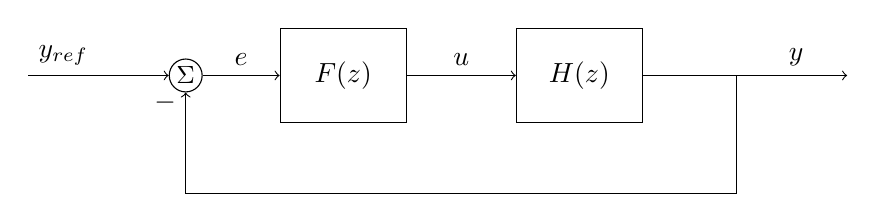
\begin{tikzpicture}[node distance = 2cm]
    \node[coordinate, ] (refinput) {};
    \node[circle, draw, inner sep=1pt, right of=refinput] (sum) {\small $\Sigma$};
    \node[draw, right of=sum, minimum height=12mm, minimum width=16mm] (controller) {$F(z)$};
    \node[draw, right of=controller, minimum height=12mm, minimum width=16mm, node distance=3cm] (plant) {$H(z)$};
    \node[coordinate, right of=plant] (measure) {};
    \node[coordinate, right of=measure,  node distance=14mm] (output) {};
    
    \draw[->] (refinput) -- node[above, near start] {$y_{ref}$} (sum);
    \draw[->] (controller) -- node[above] {$u$} (plant);
    \draw[->] (sum) -- node[above] {$e$} (controller);
    \draw[->] (plant) -- node[above, near end] {$y$} (output);
    \draw[->] (measure) -- ++(0cm, -15mm) -| node[left, pos=0.95] {$-$} (sum);

  \end{tikzpicture}
\end{center}

\abc
Using Mason's rule we get
\[ H_e(z) = \frac{1}{1 + H(z)F(z)} = \frac{1}{1 + 0.4\frac{z-0.8}{z-0.2}\frac{z+1}{(z-1)^2}} = \frac{(z-0.2)(z-1)^2}{(z-0.2)(z-1)^2 + 0.4(z-0.8)(z+1)}.\]

\abc 
The static gain is $H_e(1) = 0$. So a step-change in $y_{ref}$ will give no steady-state error. 

\abc
Using the shift operator \shift, we can write the control law as
\[ u(k) = 0.4\frac{\shift-0.8}{\shift-0.2}e(k)\]
\[ (\shift -0.2) u(k) = 0.4(\shift -0.8) e(k)\]
\[ u(k+1) - 0.2u(k) = 0.4e(k+1) - 0.32e(k)\]
\[ u(k+1) = 0.2u(k) + 0.4e(k+1) - 0.32e(k),\]
with $e(k) = y_{ref}(k) - y(k)$.

\end{exercise}

\begin{exercise}
The correct response is \textbf{III}. The reference signal is a sum of two delayed and scaled pulses, and can be written $y_{ref}(k) = \delta(k-4) + 0.3\delta(k-14)$. Correspondingly, the output should look like the superposition of two delayed and scaled pulse-responses. Responses I and IV starts at the wrong time, and can be excluded. Response II starts at $k=4$, and starts out looking correct. However, the superposed pulse response starting at $k=14$ is negative. This leaves response III as the correct response.
 
\end{exercise}

\end{document}
